\documentclass[tikz,border=10pt]{standalone}
\usepackage{pgfplots}
\usetikzlibrary{arrows.meta, positioning, calc}

\begin{document}

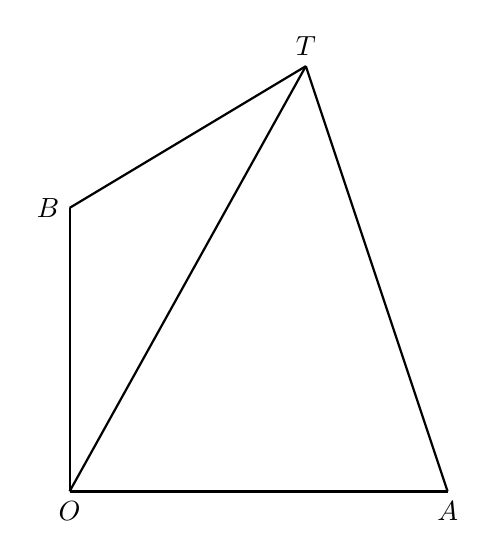
\begin{tikzpicture}[
    scale=1.2, 
    important line/.style={thick},
    point/.style={circle, fill=black, inner sep=1pt}
]
    % 1. 定义坐标点 (基于视觉比例推算)
    \coordinate (O) at (0, 0);
    \coordinate (A) at (4, 0);
    \coordinate (B) at (0, 3);
    \coordinate (T) at (2.5, 4.5);

    % 2. 绘制外边界和内部连线
    \draw[important line] (O) -- (A) node[below] {$A$};
    \draw[important line] (A) -- (T) node[above] {$T$};
    \draw[important line] (T) -- (B) node[left]  {$B$};
    \draw[important line] (B) -- (O) node[below] {$O$};
    
    % 3. 绘制内部辅助线 OT
    \draw[important line] (O) -- (T);

    % 4. 标注顶点标签 (已经包含在 draw 命令中)
    % 如果需要明确标注圆点，可以取消下面注释：
    % \foreach \p in {O,A,B,T} \fill (\p) circle (1.5pt);

\end{tikzpicture}

\end{document}